\chapter{Aerodinâmica}

\section{Dimensionamento da hélice}

Para o dimensionamento da hélice, inicialmente calculou-se o valor do parâmetro adimensional $j = \frac{V}{nD}$, onde $V$ é a velocidade de cruzeiro, $n$ é a frequência de rotação da hélice e $D$ é o diâmetro. Sabendo que a velocidade da ponta da hélice é dada por
\begin{equation}
V_\text{tip} = \sqrt{(n \pi D)^2+V^2}
\end{equation}
podemos escrever
\begin{equation}
j= \pi\frac{V}{\sqrt{V_\text{tip}-V^2}}
\end{equation}
Considerando que a velocidade da ponta é limitada por perdas de compressibilidade, o número de mach da ponta será limitado a 0,75.

Na condição de cruzeiro, $V=140\si{m/s}$ e a velocidade do som é $a=310\si{m/s}$. O valor de $j$ é então 2,37.

Para obter-se eficiência na faixa de 85\%, selecionou-se uma hélice hexa-pá. De acordo com a \autoref{fig:naca-helice}, a eficiência da hélice para esse valor de $j$ é de 86\% e o coeficiente de tração $T_c = 0,03$. O coeficiente de tração é definido
\begin{equation}
T_c = \frac{\eta P}{\rho D^2 V^3}
\end{equation}
onde $\eta$ é a eficiência da hélice, $P$ é a potência desenvolvida e $D$ é o diâmetro da hélice. Resolvendo essa equação para o diâmetro, temos
\begin{equation}
\label{eqn:D_helice}
D = \sqrt{\frac{\eta P}{\rho V^3 T_c}}
\end{equation}

\begin{figure}[H]
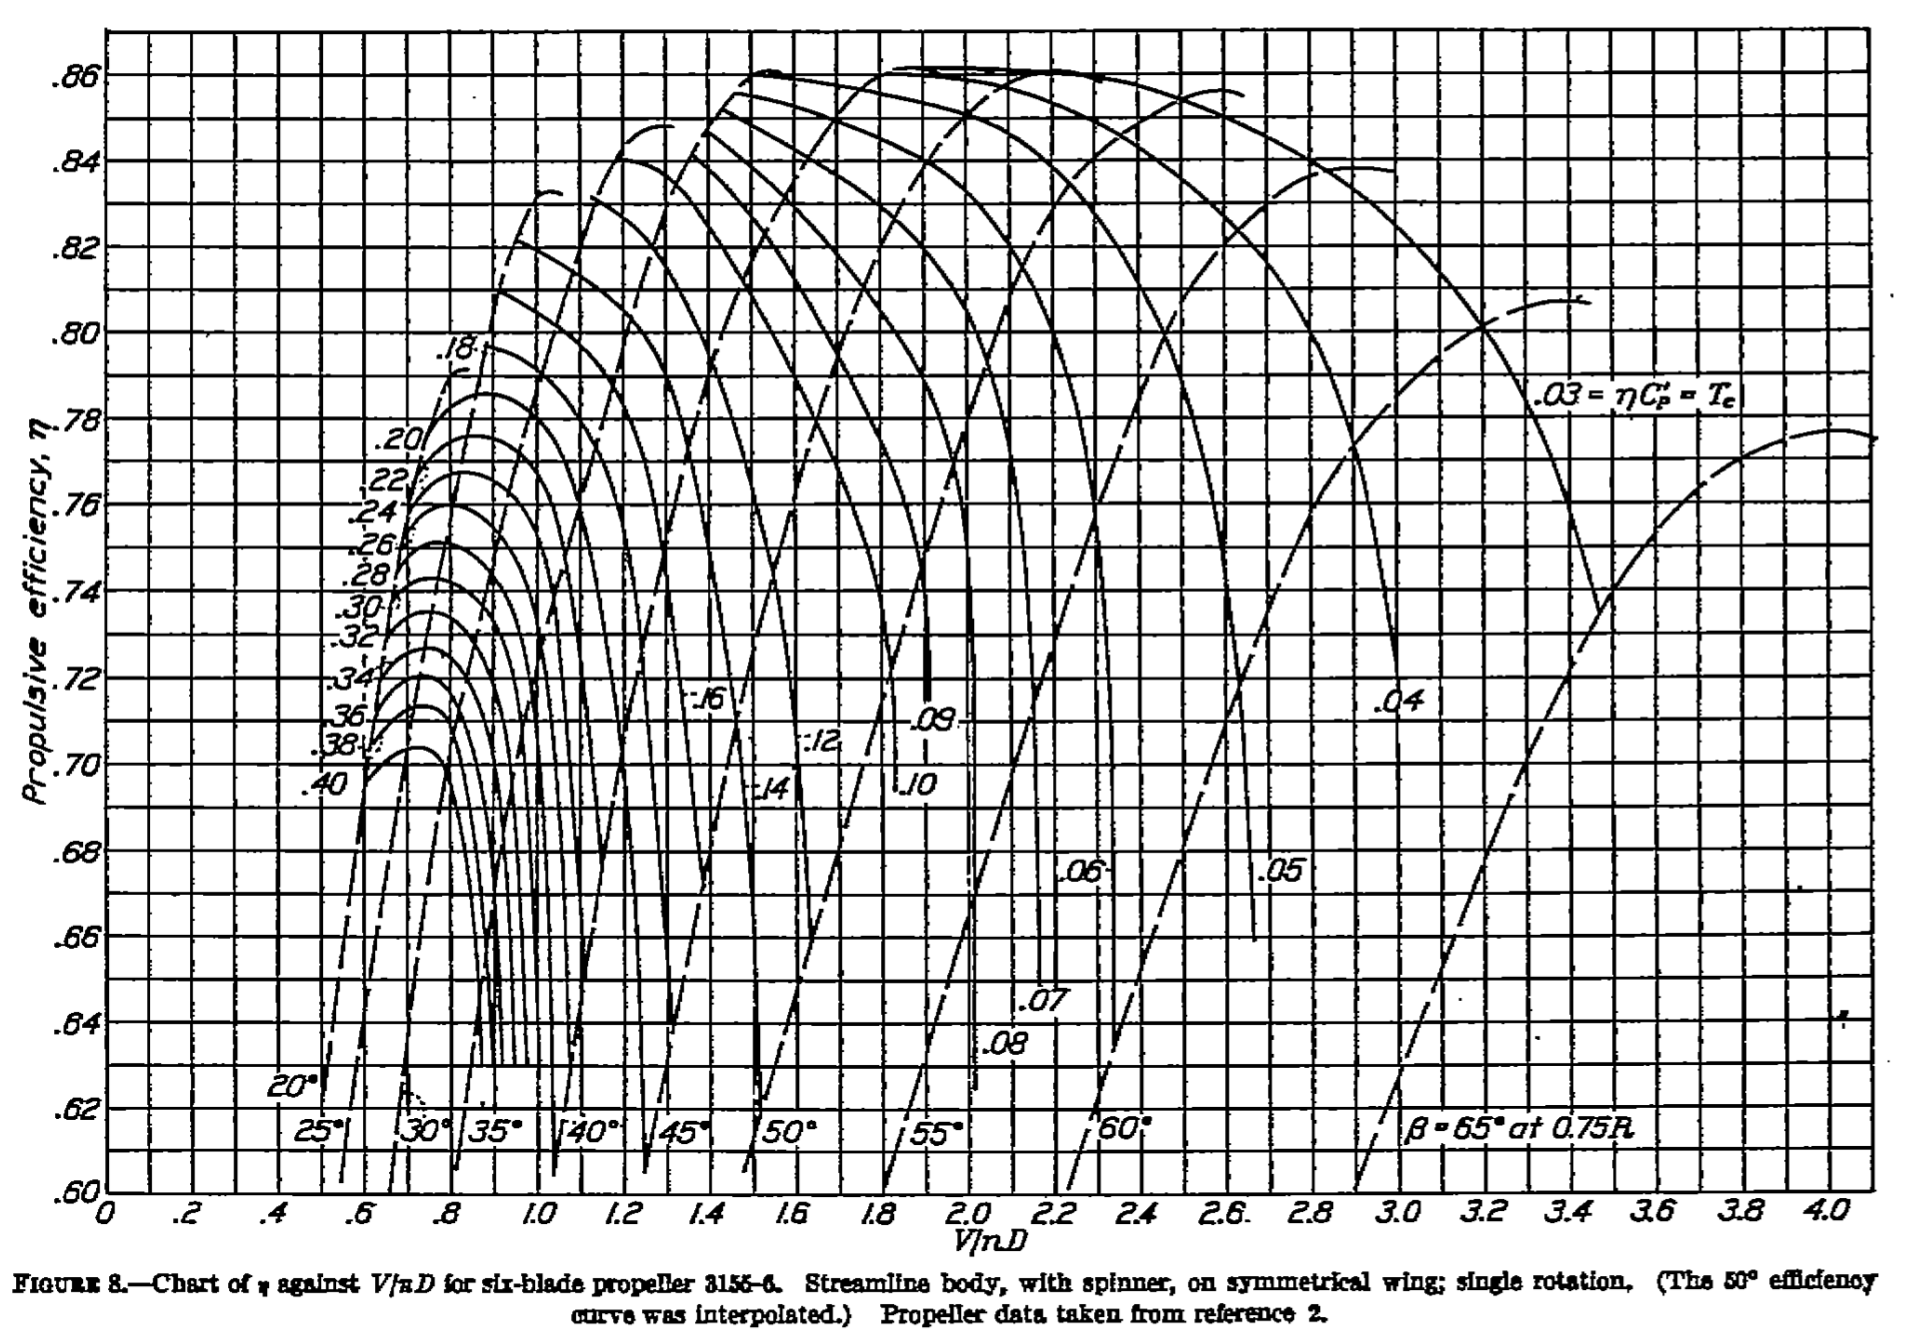
\includegraphics[width=\textwidth]{naca-helice}
\caption{Desempenho de hélice hexa-pá}  % \cite{naca-helice}
\label{fig:naca-helice}
\end{figure}

A potência requerida de decolagem é de 1383\si{kW}, ou seja, 692,5kW por hélice. Substituindo os valores na \autoref{eqn:D_helice}, o diâmetro final fica de
\begin{equation}
D=4,226\si{m}
\end{equation}

Esse diâmetro é aproximadamente duas vezes o diâmetro da fuselagem, de 2,1\si{m}, então não há risco de interferência da hélice com o solo.

%Potencia no cruzeiro: 1383kW (requerida) 2108kW (disponivel) para as duas helices

%Potencia na subida: 3692kW (dimensionante do motor)



\section{Superfícies Sustentadoras}
\label{superf_sustentadoras}

Após a definição do ponto de projeto, forma em planta da asa e das empenagens, realizou-se a modelagem aerodinâmica das superfícies sustentadoras a fim de quantificar a polar de arrasto de cada uma bem como seu $C_{L_{max}}$. Além disso, o cálculo das principais derivadas longitudinais foram determinadas iterativamente com a análise de estabilidade e controle longitudinal visto que as empenagens tiveram suas geometrias refinadas. Utilizou-se os ábacos disponiveis em ETKIN, o software XFOIL para determinação das polares 2D e o software CEA-VLM desenvolvido pelo CEA-UFMG para determinação das polares 3D. As Seções \ref{asa}, \ref{eh} e \ref{ev}  apresentam as curvas $C_L$ x $\alpha$ e as polares de arrasto. O perfil escolhido para as empenagens é o NACA0012 visto que este é um perfil típico para esta aplicação.

\subsection{Asa}
\label{asa}
A forma em planta da asa foi definida na \autoref{formaemplanta_asa} como sendo trapezoidal. Decidiu-se que o afilamento é em relação ao bordo de ataque, ou seja, não há enflechamento em relação ao bordo de ataque da asa. Essa escolha é devido a maior facilidade em posicionar o motor de forma a garantir que todo bordo de ataque da asa esteja a uma distância constante segura da hélice. Esta geometria implica que o centro aerodinâmico (CA) da asa seja mais a frente do que uma asa com afilamento em relação ao um quarto de corda visto que a corda média aerodinâmica estará posicionada mais a frente.

A asa foi modelada utilizando o software CEA-VLM. Abaixo tem-se os paineis gerados pelo código em MATLAB para asa onde é mostrado a forma em planta final da asa definida a partir da \autoref{tbl:asa_trapezoidal} e da decisão de projeto descrita acima.

\begin{figure}[H]
\centering
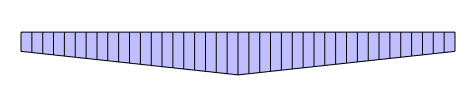
\includegraphics[width=1\textwidth]{images/parte3/malha_asa.PNG}
\caption[Paineis aerodinâmicos - Asa]{Paineis aerodinâmicos - Asa}
\label{fig:malha_asa}
\end{figure}

A partir do modelo aerodinâmico, foi possível analisar a curva de $C_L$ x $\alpha$ e polar de arrasto para asa mostrados nas figuras \ref{fig:asa_cl_alfa} e \ref{fig:asa_cl_cd}. Como descrito na \autoref{perfilasa}, o objetivo predominante na escolha do perfil da asa é a redução de arrasto, dessa forma, o perfil escolhido é de escoamento laminar com espessura máxima relativa de 18\%. Além disso, o alongamento da asa é superior ao valor típico encontrado para turboélices. A combinação dessas características permitem uma polar de arrasto competitiva para a asa sem prejudicar o projeto estrutural visto que, apesar de um alongamento maior, o perfil laminar apresenta uma espessura máxima relativa alta.

\begin{figure}[H]
\centering
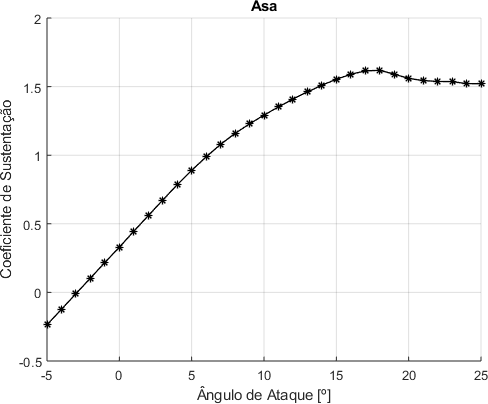
\includegraphics[width=0.75\textwidth]{images/parte3/asa_cl_alfa.png}
\caption[Curva $C_L$ x $\alpha$ para a Asa]{Curva $C_L$ x $\alpha$ para a asa}
\label{fig:asa_cl_alfa}
\end{figure}

\begin{figure}[H]
\centering
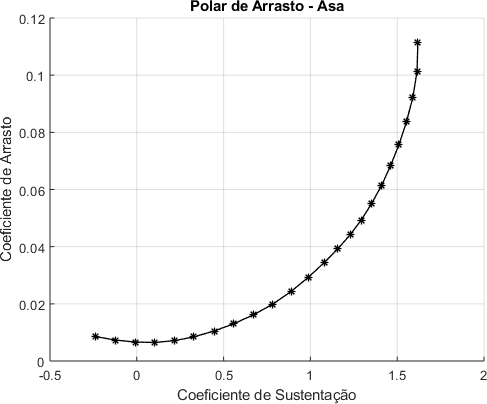
\includegraphics[width=0.75\textwidth]{images/parte3/asa_cl_cd.png}
\caption[Polar de arrasto para a Asa]{Polar de arrasto para a asa}
\label{fig:asa_cl_cd}
\end{figure}

A \autoref{tbl:resultados_asa} resume os principais resultados da análise aerodinâmica para a asa. Como pode ser observado, a variação do coeficiente de sustentação com ângulo de ataque para a asa finita se aproxima do valor calculado para o perfil. Isso era esperado dado o maior alongamento da asa. O centro aerodinâmico da asa em relaçao a corda média aerodinâmica é a 18\% sendo uma consequência da forma em planta da asa. O $C_{L_{max}}$ é 1.619 sendo o ângulo de ataque de estol correspondente 18°. Por fim o $C_{L_0}$ , $C_{M_0}$ e $C_{M_{\alpha}}$ também são apresentados.

\begin{table}[H]
\centering
\begin{tabular}{cc}
\toprule
$ \frac{\partial c_{l}}{\partial \alpha} $ & 4.740 \\ [0.3cm]
$ \frac{\partial C_{L}}{\partial \alpha} $ & 4.586 \\ [0.3cm]
$ C_{L_{max}} $ & 1.619 \\ [0.3cm]
$ \alpha_{estol} $ & 18\textdegree\ \\ [0.3cm]
$ C_{L_0} $ & 0.3293 \\ [0.3cm]
$ C_{M_0} $ & -0.0447 \\ [0.3cm]
$ C_{M_{\alpha}} $ & 0.3196 \\ [0.3cm]
$ x_{CA}/cma $ & 0.1803 \\ [0.3cm]
\bottomrule
\end{tabular}
\caption[Resultados - Asa]{Resultados - Asa}
\label{tbl:resultados_asa}
\end{table}

\subsection{Empenagem Horizontal}
\label{eh}

A área e volume de cauda da empenagem horizontal foram definidos na \autoref{formaemplanta_empenagens}. A sua forma em planta foi escolhida como trapezoidal visto que essa geometria é típica para aeronaves turboélices além de proporcionar um comportamento similar a uma forma em planta elíptica sem aumentar a complexidade na fabricação. Os valores utilizados para alogamento e afilamento \cite{gudmundsson} estão apresentados na \autoref{tbl:AR_eh} e são próximos aos valores encontrados para a aeronave DASH 8 Q400 \cite{gudmundsson}. O alongamento típico para a empenagem horizontal geralmente é entre 3 e 5. O valor baixo de alogamento é devido a uma decisão de projeto para melhorar as características de estol da empenagem horizontal evitando, por exemplo, um estol abrupto.

\begin{table}[H]
\centering
\begin{tabular}{cc}
\toprule
$ AR $ & 3.5 \\
$ \lambda_{EH} $ & 0.77 \\
\bottomrule
\end{tabular}
\caption[Alongamento e Afilamento - Empenagem Horizontal]{Alongamento e Afilamento - Empenagem Horizontal}
\label{tbl:AR_eh}
\end{table}

O valor para a distância entre o centro aerodinâmico da asa e da empenagem foi atualizado bem como o volume de cauda e área da empenagem devido a análise de estabilidade realizada no \autoref{estabilidade}. A \autoref{tbl:geometria_eh} apresenta os valores atualizados de $l_t$, $S_{eh}$, $\overline{V}_{eh}$, cordas na raiz e na ponta e a envergadura final da empenagem horizontal.

\begin{table}[H]
\centering
\begin{tabular}{cc}
\toprule
$ l_t $ & 12.255 m \\
$ S_{eh} $ & 8.9 $m^2$ \\
$ \overline{V}_{eh} $ & 1.2 \\
$ c_{raiz} $ & 1.94 m \\
$ c_{ponta} $ & 1.49 m \\
$ b $ & 5.19 m \\
\bottomrule
\end{tabular}
\caption[Geometria refinida - Empenagem Horizontal]{Geometria refinida - Empenagem Horizontal}
\label{tbl:geometria_eh}
\end{table}


A partir da \autoref{tbl:geometria_eh}, tem-se os paineis gerados pelo software CEA-VLM na \autoref{fig:malha_eh} em que é mostrado a forma em planta da empenagem horizontal.

\begin{figure}[H]
\centering
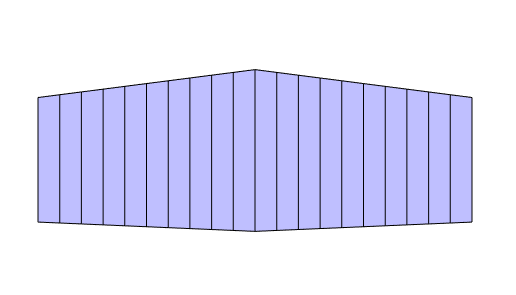
\includegraphics[width=0.45\textwidth]{images/parte3/malha_eh.PNG}
\caption[Paineis aerodinâmicos - Empenagem Horizontal]{Paineis aerodinâmicos - Empenagem Horizontal}
\label{fig:malha_eh}
\end{figure}

A partir do modelo aerodinâmico, foi possível analisar a curva de $C_L$ x $\alpha$ e polar de arrasto para empenagem horizontal mostrados nas figuras \ref{fig:eh_cl_alfa} e \ref{fig:eh_cl_cd}. Estas informações são necessárias para a análise de estabilidade realizada no \autoref{estabilidade}.

\begin{figure}[H]
\centering
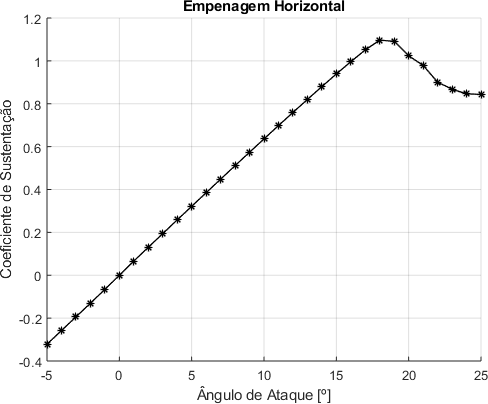
\includegraphics[width=0.75\textwidth]{images/parte3/eh_cl_alfa.png}
\caption[Curva $C_L$ x $\alpha$ para a Empenagem Horizontal]{Curva $C_L$ x $\alpha$ para a Empenagem Horizontal}
\label{fig:eh_cl_alfa}
\end{figure}

\begin{figure}[H]
\centering
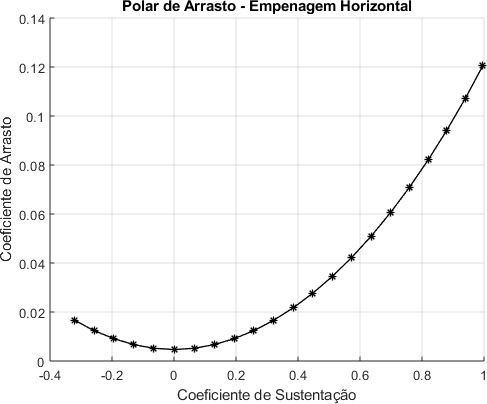
\includegraphics[width=0.75\textwidth]{images/parte3/eh_cl_cd.png}
\caption[Polar de arrasto para a Empenagem Horizontal]{Polar de arrasto para a Empenagem Horizontal}
\label{fig:eh_cl_cd}
\end{figure}

A \autoref{tbl:resultados_eh} resume os principais resultados da análise aerodinâmica para a empenagem horizontal. Como pode ser observado, a variação do coeficiente de sustentação com ângulo de ataque para a empenagem finita é menor que valor calculado para o perfil. Isso era esperado dado o menor alongamento da empenagem definido de forma a melhorar características de estol. O $C_{L_{max}}$ é 1.097 sendo o ângulo de ataque de estol correspondente 18°.

\begin{table}[H]
\centering
\begin{tabular}{cc}
\toprule
$ \frac{\partial C_{l}}{\partial \alpha} $ & 4.721 \\ [0.3cm]
$ \frac{\partial C_{L}}{\partial \alpha} $ & 3.567 \\ [0.3cm]
$ C_{L_{max}} $ & 1.097 \\ [0.3cm]
$ \alpha_{estol} $ & 18\textdegree\ \\ [0.3cm]
\bottomrule
\end{tabular}
\caption[Resultados - Empenagem Horizontal]{Resultados - Empenagem Horizontal}
\label{tbl:resultados_eh}
\end{table}

\subsection{Empenagem Vertical}
\label{ev}

A área e volume de cauda da empenagem vertical foram definidos na \autoref{formaemplanta_empenagens}. A sua forma em planta foi escolhida como trapezoidal visto que essa geometria é típica para aeronaves turboélices. Os valores utilizados para alogamento e afilamento \cite{gudmundsson} estão apresentados na \autoref{tbl:AR_ev} e são próximos aos valores encontrados para a aeronave DASH 8 Q400. O alongamento típico para a empenagem vertical geralmente é entre 1 e 2.

\begin{table}[H]
\centering
\begin{tabular}{cc}
\toprule
$ AR $ & 1.4 \\
$ \lambda_{EV} $ & 0.71 \\
\bottomrule
\end{tabular}
\caption[Alongamento e Afilamento - Empenagem Vertical]{Alongamento e Afilamento - Empenagem Vertical}
\label{tbl:AR_ev}
\end{table}


O valor para a distância entre o centro aerodinâmico da asa e da empenagem foi atualizado bem como o volume de cauda e área da empenagem. A \autoref{tbl:geometria_ev} apresenta os valores atualizados de $S_{ev}$, $\overline{V}_{ev}$, cordas na raiz e na ponta e a envergadura final da empenagem horizontal. O enflechamento em relação a um quarto de corda foi definido como 20°.

\begin{table}[H]
\centering
\begin{tabular}{cc}
\toprule
$ S_{ev} $ & 11.89 $m^2$ \\
$ \overline{V}_{ev} $ & 1.2 \\
$ c_{raiz} $ & 3.41 m \\
$ c_{ponta} $ & 2.42 m \\
$ b $ & 4.08 m \\
$ Enflechamento $ & 20° \\
\bottomrule
\end{tabular}
\caption[Geometria refinada - Empenagem Vertical]{Geometria refinida - Empenagem Vertical}
\label{tbl:geometria_ev}
\end{table}

A partir da \autoref{tbl:geometria_ev}, tem-se os paineis gerados pelo software CEA-VLM na \autoref{fig:malha_eh} em que é mostrado a forma em planta da empenagem vertical.


\begin{figure}[H]
\centering
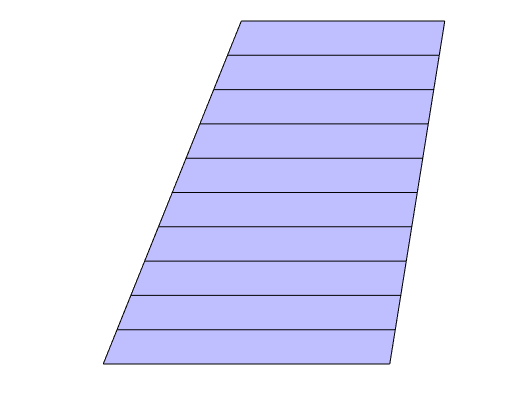
\includegraphics[width=0.45\textwidth]{images/parte3/malha_ev.PNG}
\caption[Paineis aerodinâmicos - Empenagem Vertical]{Paineis aerodinâmicos - Empenagem Vertical}
\label{fig:malha_ev}
\end{figure}

A partir do modelo aerodinâmico, foi possível analisar a curva de $C_L$ x $\alpha$ e polar de arrasto para empenagem vertical mostrados nas figuras \ref{fig:ev_cl_alfa} e \ref{fig:ev_cl_cd}.

\begin{figure}[H]
\centering
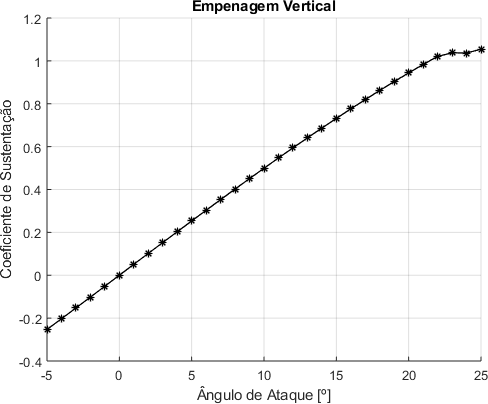
\includegraphics[width=0.75\textwidth]{images/parte3/ev_cl_alfa.png}
\caption[Curva $C_L$ x $\alpha$ para a Empenagem Vertical]{Curva $C_L$ x $\alpha$ para a Empenagem Vertical}
\label{fig:ev_cl_alfa}
\end{figure}

\begin{figure}[H]
\centering
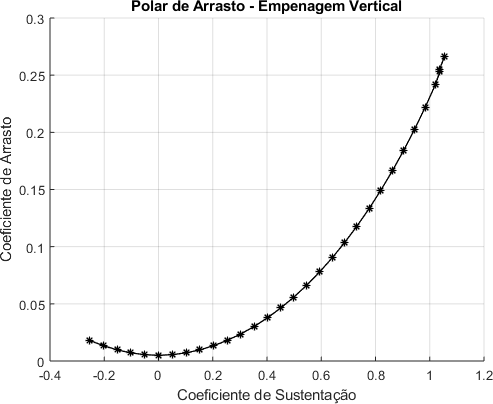
\includegraphics[width=0.75\textwidth]{images/parte3/ev_cl_cd.png}
\caption[Polar de arrasto para a Empenagem Vertical]{Polar de arrasto para a Empenagem Vertical}
\label{fig:ev_cl_cd}
\end{figure}

A \autoref{tbl:resultados_ev} resume os principais resultados da análise aerodinâmica para a empenagem vertical. Como pode ser observado, a variação do coeficiente de sustentação com ângulo de ataque para a empenagem finita é consideravelmente menor que valor calculado para o perfil. Isso era esperado dado o menor alongamento da empenagem definido de forma a melhorar características de estol. O $C_{L_{max}}$ é 1.097 sendo o ângulo de ataque de estol correspondente 23°.

\begin{table}[H]
\centering
\begin{tabular}{cc}
\toprule
$ \frac{\partial C_{l}}{\partial \alpha} $ & 4.721 \\ [0.3cm]
$ \frac{\partial C_{L}}{\partial \alpha} $ & 2.630 \\ [0.3cm]
$ C_{L_{max}} $ & 1.054 \\ [0.3cm]
$ \alpha_{estol} $ & 23\textdegree\ \\ [0.3cm]
\bottomrule
\end{tabular}
\caption[Resultados - Empenagem Vertical]{Resultados - Empenagem Vertical}
\label{tbl:resultados_ev}
\end{table}

\section{Superficies hipersustentadoras}
Para os cálculos iniciais de desempenho, apresentados no \autoref{diagramarestricoes}, foi considerado que o coeficiente de sustentação máximo da asa era de 2.
Agora, com os cálculos refinados de aerodinâmica apresentados neste capítulo, o $C_L$ máximo da asa é, na verdade, de 1,62.
Isso significa que, para a decolagem e pouso, o valor desse coeficiente deve ser aumentado em pelo menos 0,4 durante pousos e decolagens para cumprir com os requisitos estipulados para a missão.
Como a geometria da asa foi otimizada para cruzeiro, ela não deve ser modificada para essa fase de voo.
A solução é utilizar uma asa de geometria variável, através do uso de superfícies hipersustentadoras: flaps e slats.

De acordo com os dados apresentados em \cite{gudmundsson}, é relativamente fácil conseguir esse aumento em $C_L$.
O uso de flaps simples (``\emph{plain flaps}'')  isoladamente já cumpriria com esse requisito.
O projeto aqui apresentado não se contentará com isso e procurará especificar o melhor sistema de hipersustentação possível, o que poderá ser usado para aumentar o $C_L$ máximo em iterações futuras e melhorar o desempenho da aeronave, possívelmente alterando seu ponto de projeto.

\subsection{Slats}
O slat a ser utilizado é um de três posições (pouso, decolagem e retraído).
A posição para pouso é escolhida para maximizar a sustentação e causa grande aumento de arrasto, o que torna o pouso mais controlado.
A de decolagem é projetada para maximizar o desempenho de subida.

De acordo com \cite{gudmundsson}, um flap desse tipo traz ganhos de
\begin{align}
    \Delta {C_l}_{\max} &\approx {0,84} \\
    \Delta {\alpha}_{\max} &\approx \ang{11} \\
    \Delta {C_d}_{\min} &\approx 80\cdot 10^{-4} \\
    \Delta {C_m} &\approx -{0,115}
\end{align}
A deflexão dos slats é de aproximadamente \ang{25}.

\subsection{Flaps}
Para aeronaves de transporte, o usual é a utilização de \emph{flaps fowler} com uma ou duas fendas (``\emph{slots}'').
Esse tipo de flap proporciona ganhos bastante elevados em $C_L$ e a opção de ganhos moderados ou grandes em arrasto, dependendo da configuração (decolagem ou pouso).
Para este projeto, o \emph{flap fowler} de uma fenda foi preferido devido à sua maior simplicidade construtiva, e a não haver necessidade dos ganhos de $C_L$ superiores que podem ser obtidos usando mais fendas.

De acordo com \cite{gudmundsson}, os ganhos esperados são de
\begin{align*}
    \Delta {C_l}_{\max}|_{\text{decolagem}} &\approx 1,16 \\
    \Delta {C_l}_{\max}|_{\text{pouso}} &\approx 1,92 \\
    \Delta {\alpha}_{\max} &\approx \ang{-7} \\
    \Delta {C_d}_{\min} &\approx 40\cdot 10^{-4} \\
    \Delta {C_m} &\approx -0,75
\end{align*}
A deflexão de decolagem é de \ang{15} e a de pouso é de \ang{40}.

\subsection{Novos coeficientes para a asa}
Os slats deverão ser instalados por toda a extensão da asa.
Os flaps obviamente não podem ser instalados no mesmo lugar dos ailerons, então só irão até essas
superfícies de controle.
Isso tem o benefício adicional de evitar o estol de ponta com as superfícies de hipersustentação defletidas, já que, sem os flaps, o ângulo de estol da ponta de asa será substancialmente maior que o da raiz.

Considerando que o aileron vai ocupar aproximadamente 20\% da envergadura, temos
que a área flapeada é dada por
\begin{equation}
    S_{\text{flap}} = 0,8 b c_r (1+\frac{\lambda}{0,8})/2 = 45.7\si{m^2}
\end{equation}

Fazendo a média ponderada nas áreas e ignorando o arrasto induzido para uma
primeira aproximação, os novos coeficientes esperados são dados por
\begin{equation}
    C_X = {C_X}_{\text{limpo}} + \sum_i{\Delta_i C_X \frac{{S_X}_i}{S}}
\end{equation}
e os seus valores são
\begin{align*}
    {C_L}_{\max}|_{\text{decolagem}} &\approx 3.4 \\
    {C_L}_{\max}|_{\text{pouso}} &\approx 4.1\\
    {\alpha}_{\max} &\approx \ang{22} \\
    {C_d}_{\min} &\approx 151\cdot 10^{-4} \\
    {C_M} &\approx -0,80
\end{align*}

